\documentclass[11pt,letterpaper]{article}
\usepackage[utf8]{inputenc}
\usepackage{amsmath,amssymb,fullpage,graphicx}
\usepackage{subfigure}
\let\hat\widehat
\let\tilde\widetilde

\begin{document}
\subsection*{Q1-a}
\noindent Let $R = (\frac{X_1 - \bar{X}}{S}, \frac{X_2 - \bar{X}}{S}... \frac{X_n - \bar{X}}{S})$. 

\noindent Since we assume $X_i$'s are from $N(\theta, \sigma^2)$, so $X_i$ can be represented by $\sigma Z_i + \theta$, and $\bar{X} = \sigma \bar{Z} + \theta$.

\noindent $S$ denotes sample standard deviation, $S = \sqrt{\frac{1}{n-1} \sum (x_i - \bar{x})^2}$ 

\begin{align*}
R_i &= \frac{\sigma(Z_i - \bar{Z})}{S} \\
&= \frac{\sigma(Z_i - \bar{Z})}{\sqrt{\frac{\sigma^2}{n-1} \sum (Z_i - \bar{Z)^2})}} \\
&= \frac{\sqrt{n-1} (Z_i - \bar{Z})}{\sqrt{\sum (Z_i - \bar{Z})^2}}
\end{align*}

\noindent Under normality assumption, $R_i$ only depends on $Z_i$.

\begin{verbatim}
sp_dt <- c(14.0, 9.4, 12.1, 13.4, 6.3, 8.5, 7.1, 12.4, 13.3, 9.1)
n <- length(sp_dt)
B = 10000
D_values <- rep(NA, B)
for (ii in 1:B) {
  sim_z <- rnorm(n=10) 
  sim_resid <- sqrt(n-1) * (sim_z - mean(sim_z)) / sqrt(sum((sim_z - mean(sim_z))^2))
  sim_D <- (n-1)^(-3/2) * sum(sim_resid^3)
  D_values[ii] <- sim_D
}
hist(D_values, probability=T, xlim=c(-1, 1), 
     xlab='D-skew values', main='Histogram of D-skew')
\end{verbatim}

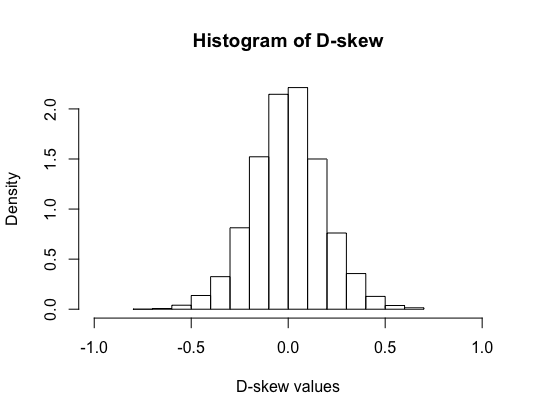
\includegraphics[scale=0.55]{q1-a.png}

\subsection*{Q1-b}
\noindent Now we get the density function of discrepancy statistic $D$, under the normal assumption of $X$. We will check whether $D-value$ of the observed sample is surprising, under this assumption by calculating its p-value. \\

\noindent Since we generated $10^4$ random $D$, the p-value is proportion of random $D$'s whose values are more extreme than observed $D$. \\

\noindent Note that $D = (n-1)^{-\frac{3}{2}} \sum_{i=1}^{n} (R_i)^3$

\noindent Where $R_i = \frac{X_i - \bar{X}}{S}$

\begin{verbatim}
sp_sd <- sd(sp_dt)
sp_resid <- sp_dt - mean(sp_dt)
ancillary_R <- sp_resid / sp_sd
sp_D <- (n-1)^(-3/2) * sum(ancillary_R^3)
p_value <- length(D_values[D_values < sp_D | D_values > abs(sp_D)]) / 10000

> sp_D
[1] -0.06364436
> p_value
[1] 0.7049
\end{verbatim}

\noindent In this case, the discrepancy statistic of observed data is $-0.06364436$, with its p-value of $0.7049$. i.e. under normality assumption, $70 \%$ of $D-values$ are more extreme than observed $D$. \\

\noindent Therefore, under the significance level of 0.05, observed data fail to show significant evidence against normality model. 











\end{document}